\documentclass[crop,tikz]{standalone}

\usepackage{pgfplots}
\tikzset{>=latex}

\pgfplotsset{
  inverted/.style = {
    every axis legend/.append style={
      draw=white,
      fill=hardblack,
      text=white
    }
  },
  every non boxed x axis/.append style={
    axis line style={-latex}
  },
  every non boxed y axis/.append style={
    axis line style={-latex}
  }
}

\begin{document}
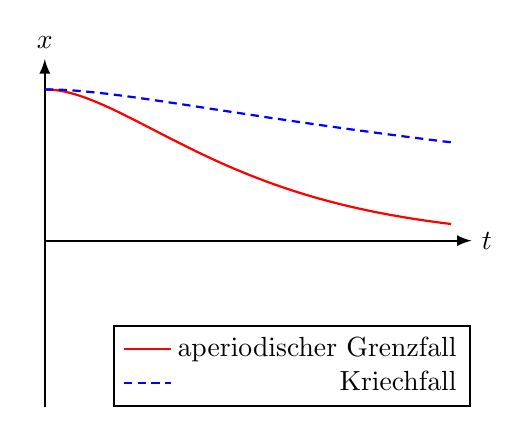
\begin{tikzpicture}
\pgfmathsetmacro{\damp}{0.2}
\pgfmathsetmacro{\apar}{1}
\pgfmathsetmacro{\bpar}{1}
\begin{axis}[
  thick,
  width=7cm,
  height=6cm,
  domain={0}:{6*pi},
  samples=50,
  axis y line=middle,
  axis x line=middle,
  xlabel={$t$},
  ylabel={$x$},
  xlabel style={right},
  ylabel style={above},
  xmin=0, xmax={6.3*pi},
  ymin=-1.1, ymax=1.2,
  xtick={\empty},
  xticklabels={\empty},
  ytick={\empty},
  yticklabels={\empty},
  legend cell align={right},
  legend style={at={(1,0)},anchor=south east}
  ]
  \addplot[red,smooth] { (\apar + \damp*x)*exp(-\damp*x) };
  \addlegendentry{aperiodischer Grenzfall};
  \addplot[blue,densely dashed,smooth] {exp(-0.2*x)*(1.07735*exp(sqrt(0.03)*x) - 0.0773503*exp(-sqrt(0.03)*x))};
  \addlegendentry{Kriechfall};
\end{axis}
\end{tikzpicture}
\end{document}
